% 1) Title
% 2) Date
% 3) Location
% 4) Present
% 5) Picture
% 6) Start Time
% 7) Stop Time
\insertmeeting 
	{More Intake} 
	{08/26/21}
	{Hagerty High School}
	{Annika, Jensen, Nathan}
	{Images/RobotPics/robot.jpg}
	{2:30}
  {4:30}
	
\section*{Hardware}
\noindent\hfil\rule{\textwidth}{.4pt}\hfil
\subsection*{Goals}
\begin{itemize}
    \item Finish putting Teflon tape on bearings
	\item Rebuild intake
	\item Test sweeper
  

\end{itemize} 

\noindent\hfil\rule{\textwidth}{.4pt}\hfil

\subsection*{Accomplishments}
In today’s meeting we resumed our work from Tuesday, continuing to cover the backs of the vex bearing blocks with Teflon tape to reduce the friction between the bearing blocks and the wooden intake plate (image1). This was a surprisingly lengthy process because of how difficult it was to create holes in the right place for screws to go through the bearings, and because the tape kept detaching from the bearings throughout the process.
While one of our members worked on putting the Teflon tape on, we had another member getting the sweeper intake ready to attach. Once the teflon tape was on and the sweeper was ready, we put all of the pieces back together and tested the intake once again, this time with the sweeper instead of the rubber band spinner (image 2). Although testing isn’t totally reliable because we still have to turn the sweeper by hand due to a shortage of vex wires, we found that at first the sweeper didn’t work as well as the rubber band intake. As we looked for possible reasons why, we found that it was the slots that were limiting the sweeper’s abilities. Although the teflon tape significantly reduced the friction, allowing whatever type of intake was attached to move up and down more freely, the sweeper wasn’t moving up and down as much as the rubber band spinner was. This, instead of being due to friction in the slots, is caused by the different shapes of the intakes. The rubber band intake is shaped more regularly, like a cylinder, and is firmer, making it easy for game elements to push against it, moving the rubber band spinner up through the slots. The sweeper on the other hand is irregularly shaped and is less firm. This means that when game elements go through it, it is harder to move through the slots and sometimes instead binds up.
Although this may be seen as a reason to use the rubber band intake instead of the sweeper, we decided to test the sweeper a bit higher in the slots and not letting it move up and down. We did this by tightening the nuts holding the bearing blocks in the slots, which held them firmly, a bit higher than they would have been just resting at the bottom of the slots (image 3). When we tested this we got much better results, finding it to work about as well as the rubber band intake. This means that for our future intake design in the upcoming season, using the sweeper might be better because even though it works similar to the rubber band intake, it doesn't need to slide up and down, simplifying and shrinking how big the mechanism would need to be. All of this still depends on the game, however, and we still need to test both intake designs with the motor to make the test more realistic to the actual game.


\begin{figure}[ht]
\centering
\begin{minipage}[b]{.50\textwidth}
  \centering
  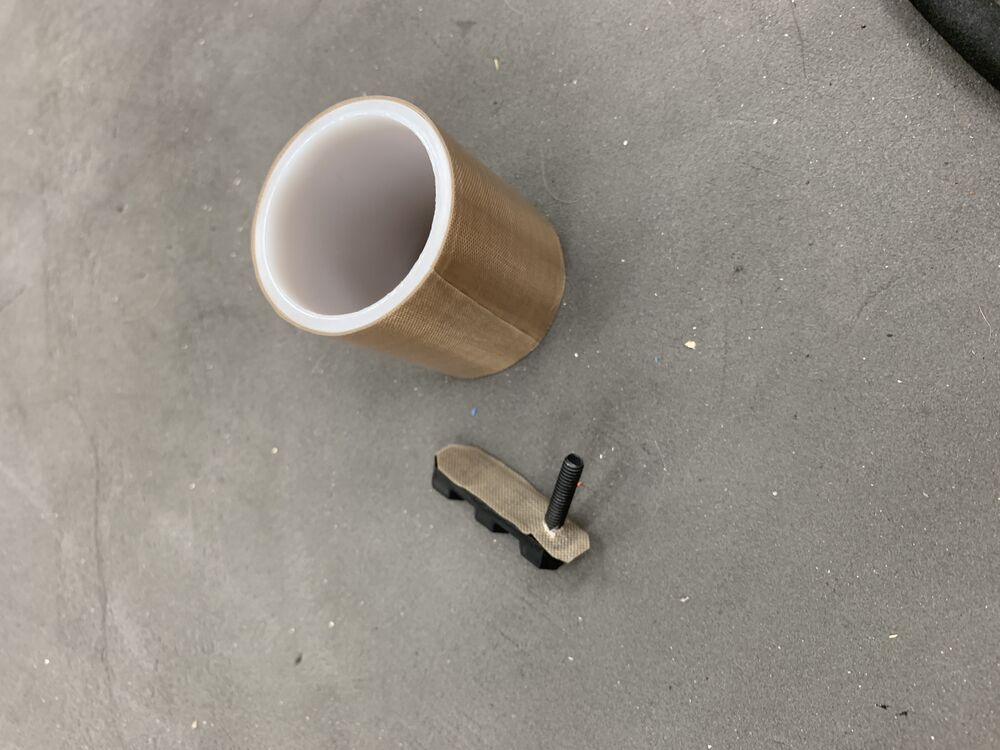
\includegraphics[width=0.8\textwidth]{Meetings/August/08-18-21/8-26-21_Hardware_Image1 - Nathan Forrer.JPG}
  \caption{Our bearing blocks covered in Teflon to reduce friction with the plates.}
  \label{fig:pic1}
\end{minipage}%
\hfill%
\begin{minipage}[b]{.50\textwidth}
  \centering
  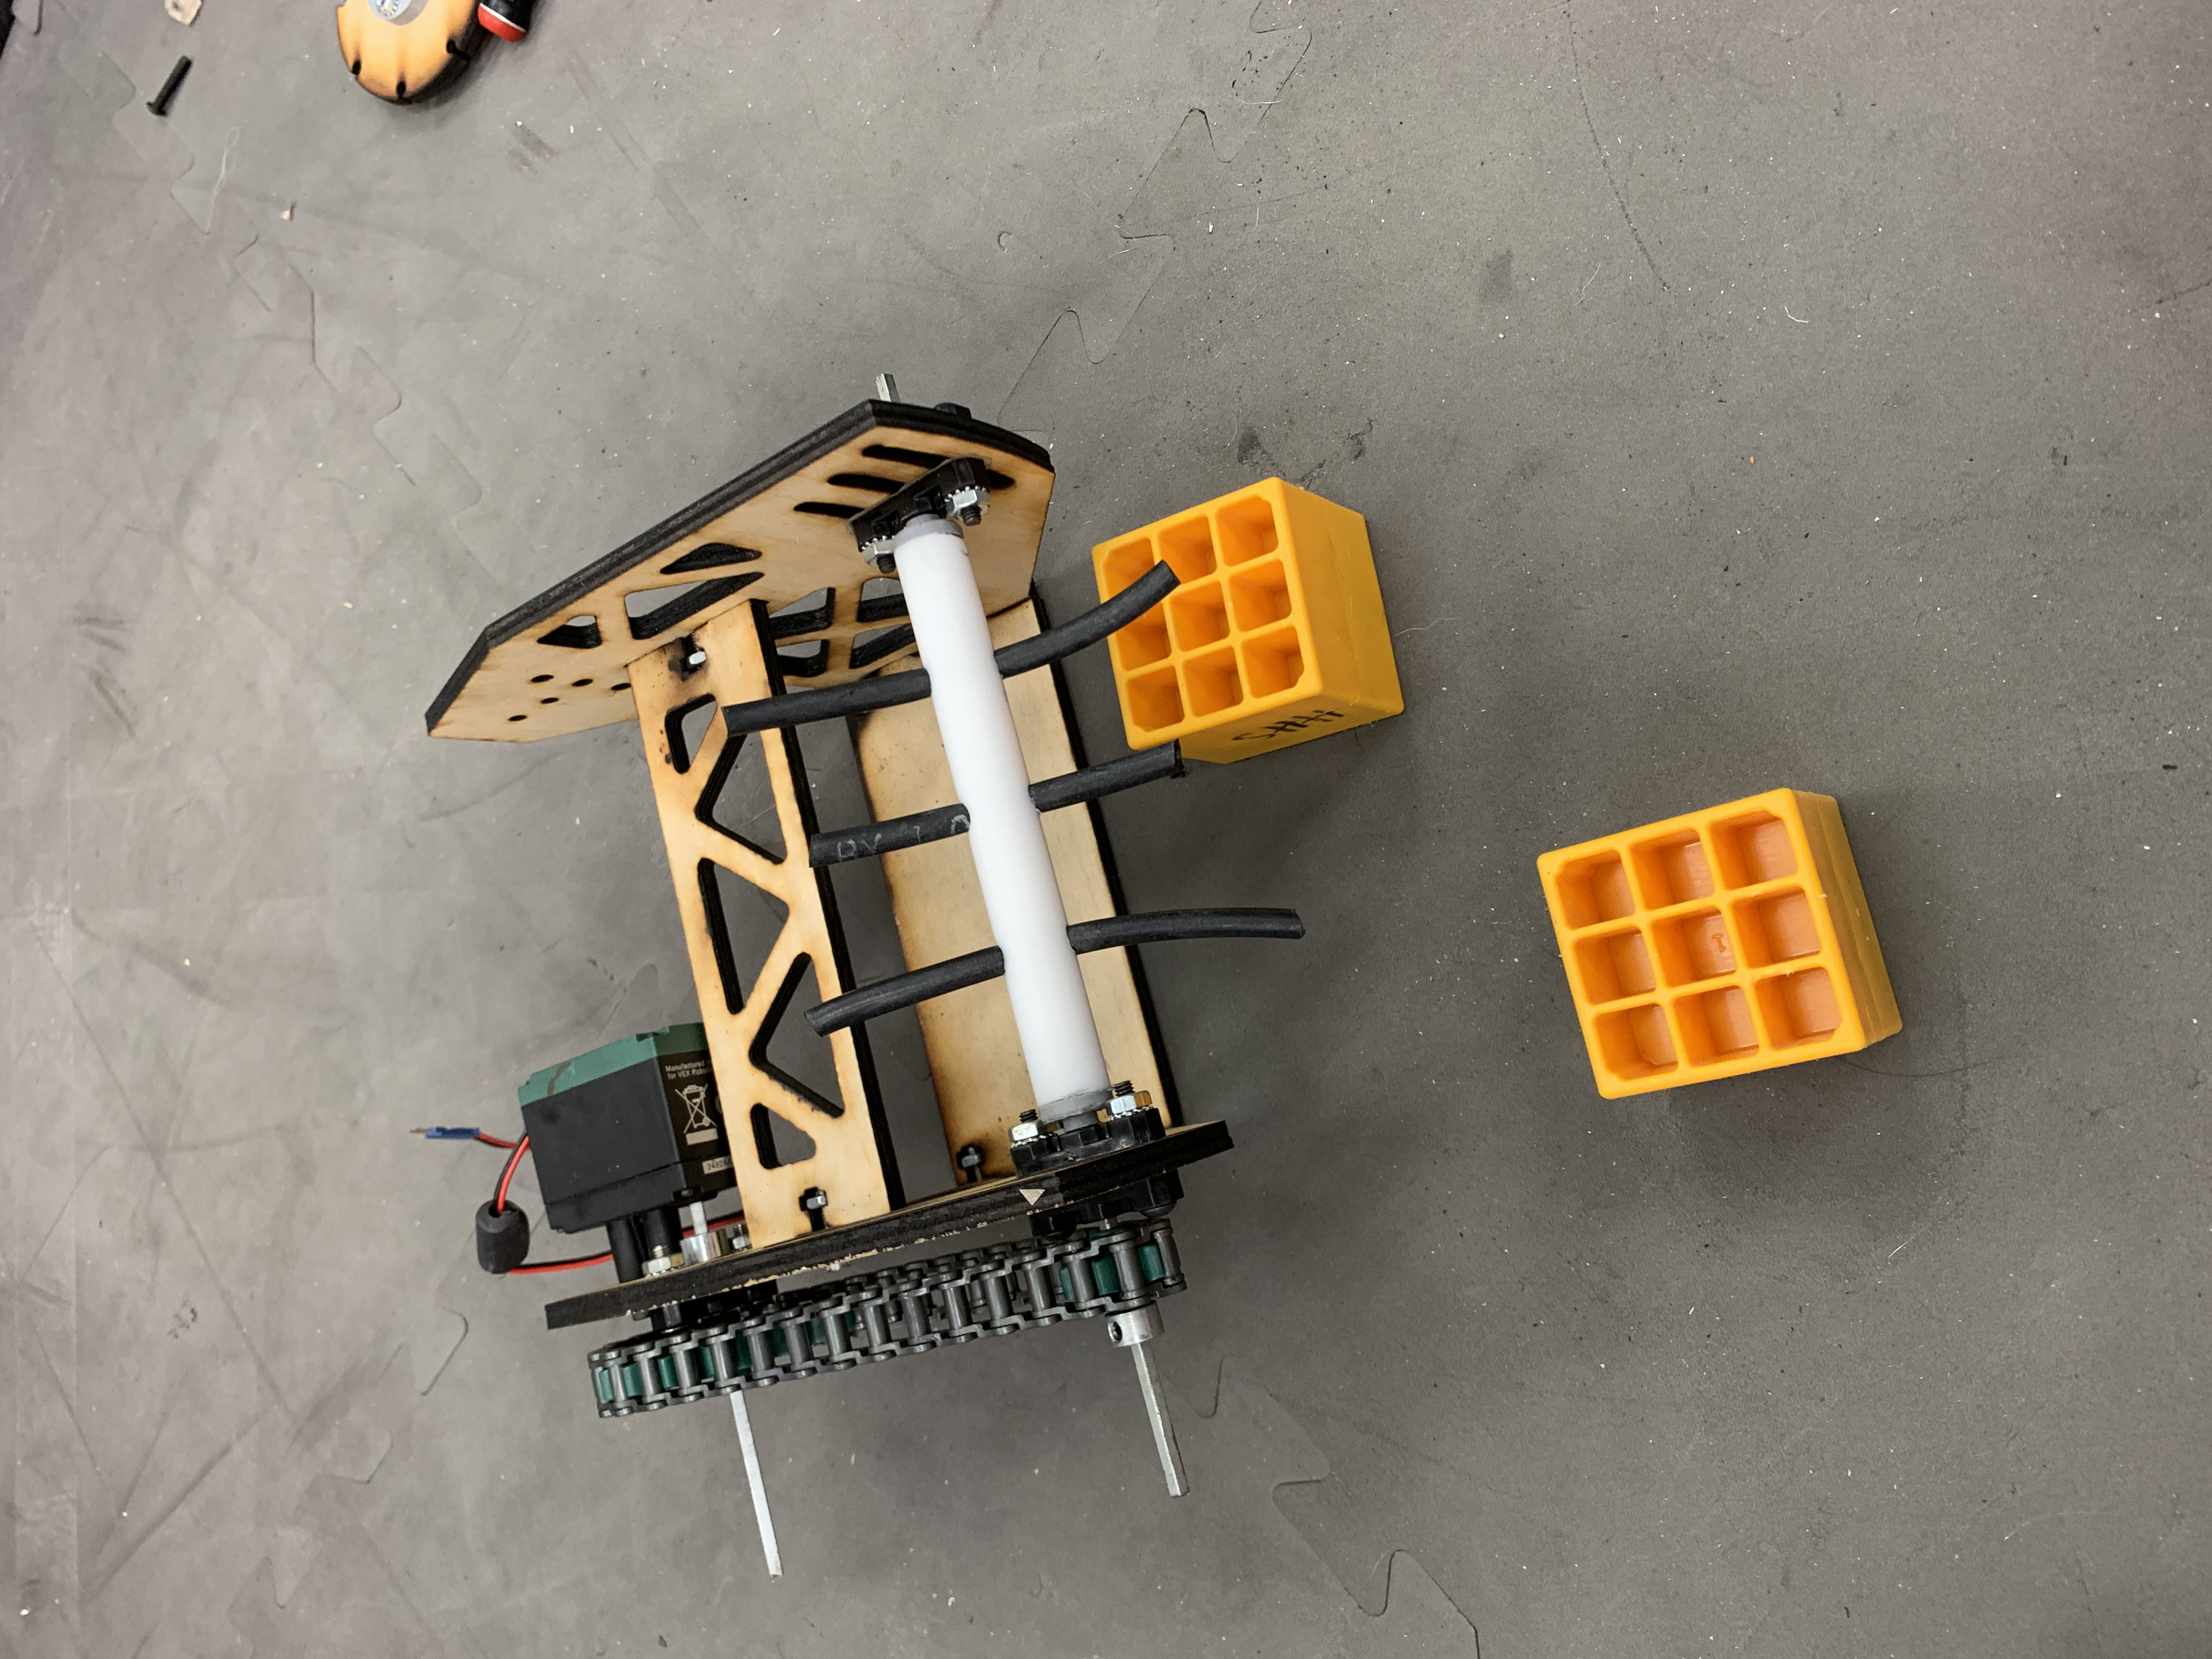
\includegraphics[width=0.8\textwidth]{Meetings/August/08-18-21/8-26-21_Hardware_Image2 - Nathan Forrer.JPG}
  \caption{Our second version of the intake uses a tube sweeper instead of the rubber band spinner.}
  \label{fig:pic2}
\end{minipage}
\end{figure}

\begin{figure}[htp]
\centering
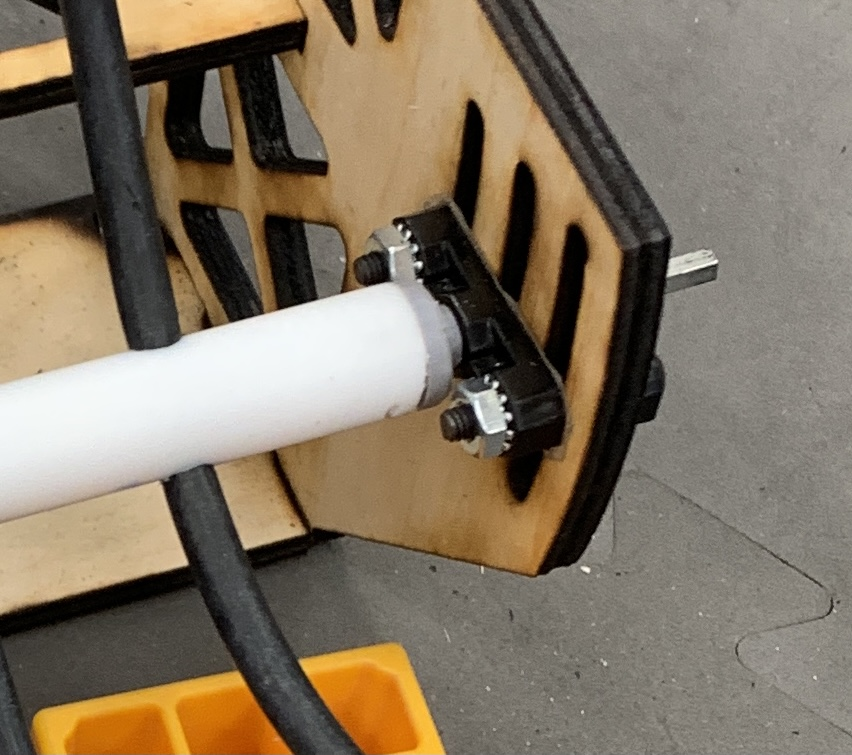
\includegraphics[width=0.8\textwidth]{Meetings/August/08-18-21/8-26-21_Hardware_Image3 - Nathan Forrer.JPG}
\caption{We got better results when tightening the nuts higher than expected.}
\label{fig:pic3}
\end{figure}